% !TeX root=main.tex
\begin{frame}[fragile]
  \frametitle{Go-Stop + AlphaZero}
  \framesubtitle{Main Goal}

  \begin{center}
  \vcenteredhbox{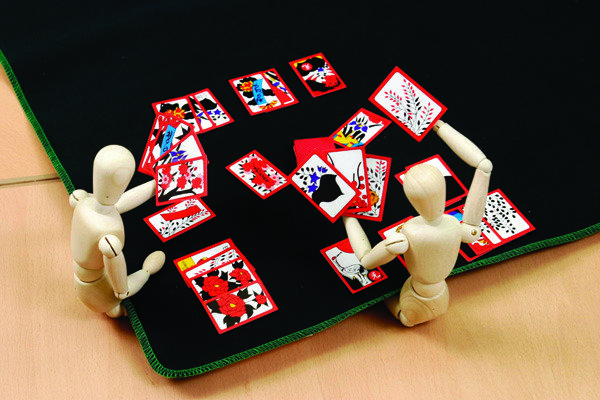
\includegraphics[width=0.4\textwidth]{images/dolls-playing-go-stop.jpg}}
  \vcenteredhbox{\fontsize{50}{50}\selectfont\,+\,}
  \vcenteredhbox{\begin{tikzpicture}
    \node[circle,
      text=white,
      minimum width=0.3\textwidth,
      path picture={
          \node at (path picture bounding box.center){
              
\includegraphics[width=0.3\textwidth]{images/deepmind-logo.jpg}
          };
      }]{};
      \node at (0,0) {\textcolor{black}{\Large\bfseries AlphaZero}};
  \end{tikzpicture}}
  \end{center}
\end{frame}

\begin{frame}[c, fragile]
  \frametitle{How to Play Go-Stop}
  \framesubtitle{Cards}

  \begin{columns}
    \begin{column}{0.55\textwidth}
      \begin{table}[]
        \begin{tabular}{ll}
          \parbox[][3.088em][c]{3em}{Jan.} & \parbox[][3.088em][c]{9em}{
            
\includegraphics[width=2em]{images/cards/B01}
            
\includegraphics[width=2em]{images/cards/R01}
            
\includegraphics[width=2em]{images/cards/J010}
            
\includegraphics[width=2em]{images/cards/J011}
          } \\[1.5em]
          \parbox[][3.088em][c]{3em}{Feb.} & \parbox[][3.088em][c]{9em}{
            
\includegraphics[width=2em]{images/cards/A02}
            
\includegraphics[width=2em]{images/cards/R02}
            
\includegraphics[width=2em]{images/cards/J020}
            
\includegraphics[width=2em]{images/cards/J021}
          } \\[1.5em]
          \parbox[][3.088em][c]{3em}{Mar.} & \parbox[][3.088em][c]{9em}{
            
\includegraphics[width=2em]{images/cards/B03}
            
\includegraphics[width=2em]{images/cards/R03}
            
\includegraphics[width=2em]{images/cards/J030}
            
\includegraphics[width=2em]{images/cards/J031}
          } \\[1.5em]
          \parbox[][3.088em][c]{3em}{Apr.} & \parbox[][3.088em][c]{9em}{
            
\includegraphics[width=2em]{images/cards/A04}
            
\includegraphics[width=2em]{images/cards/R04}
            
\includegraphics[width=2em]{images/cards/J040}
            
\includegraphics[width=2em]{images/cards/J041}
          } \\
          \parbox[][3.088em][c]{3em}{} & \parbox[][3.088em][c]{9em}{\hspace{3em}$\vdots$} \\
        \end{tabular}
      \end{table}
    \end{column}

    \begin{column}{0.45\textwidth}
      \begin{table}[]
        \begin{tabular}{ll}
        \parbox[][3.088em][c]{4.5em}{Bright} & \parbox[][3.088em][c]{4.5em}{
          
\includegraphics[width=2em]{images/cards/B11}
          
\includegraphics[width=2em]{images/cards/B08}
        }
        \parbox[][3.088em][c]{1em}{$\cdots$} \\[1.5em]
        \parbox[][3.088em][c]{4.5em}{Animal} & \parbox[][3.088em][c]{4.5em}{
          
\includegraphics[width=2em]{images/cards/A02}
          
\includegraphics[width=2em]{images/cards/A09}
        }
        \parbox[][3.088em][c]{1em}{$\cdots$} \\[1.5em]
        \parbox[][3.088em][c]{4.5em}{Ribbon} & \parbox[][3.088em][c]{4.5em}{
          
\includegraphics[width=2em]{images/cards/R04}
          
\includegraphics[width=2em]{images/cards/R06}
        }
        \parbox[][3.088em][c]{1em}{$\cdots$} \\[1.5em]
        \parbox[][3.088em][c]{4.5em}{Junk} & \parbox[][3.088em][c]{4.5em}{
          
\includegraphics[width=2em]{images/cards/J051}
          
\includegraphics[width=2em]{images/cards/J112}
        }
        \parbox[][3.088em][c]{1em}{$\cdots$} \\[1.5em]
        \parbox[][3.088em][c]{4.5em}{Bonus} & \parbox[][3.088em][c]{4.5em}{
          
\includegraphics[width=2em]{images/cards/bonus2}
          
\includegraphics[width=2em]{images/cards/bonus3}
        }
        \end{tabular}
      \end{table}
    \end{column}
  \end{columns}
\end{frame}

\begin{frame}[fragile]
  \frametitle{How to Play Go-Stop}
  \framesubtitle{Turns}

  \begin{center}
    \parbox{\textwidth}{
      \centering
      
\includegraphics[width=2em]{images/cards/hidden}
      
\includegraphics[width=2em]{images/cards/hidden}
      
\includegraphics[width=2em]{images/cards/hidden}
      
\includegraphics[width=2em]{images/cards/hidden}
      
\includegraphics[width=2em]{images/cards/hidden}
    }

    \vspace*{1.5em}

    \parbox{\textwidth}{
      \centering
      \parbox{2em}{
        
\includegraphics[width=2em]{images/cards/J011}\\
        
\includegraphics[width=2em]{images/cards/A07}
      }
      \quad
      \parbox{2em}{%
        \vspace*{0em}%
        
\includegraphics[width=2em]{images/cards/hidden}
      }
      \quad
      \parbox{2em}{
        
\includegraphics[width=2em]{images/cards/J020}\\
        
\includegraphics[width=2em]{images/cards/R04}
      }
    }

    \vspace*{1.5em}

    \parbox{\textwidth}{
      \centering
      
\includegraphics[width=2em]{images/cards/J010}
      
\includegraphics[width=2em]{images/cards/J050}
      
\includegraphics[width=2em]{images/cards/J060}
      
\includegraphics[width=2em]{images/cards/J070}
      
\includegraphics[width=2em]{images/cards/R10}
    }
  \end{center}
\end{frame}

\begin{frame}[fragile]
  \frametitle{How to Play Go-Stop}
  \framesubtitle{Turns}

  \begin{center}
    \parbox{\textwidth}{
      \centering
      
\includegraphics[width=2em]{images/cards/hidden}
      
\includegraphics[width=2em]{images/cards/hidden}
      
\includegraphics[width=2em]{images/cards/hidden}
      
\includegraphics[width=2em]{images/cards/hidden}
      
\includegraphics[width=2em]{images/cards/hidden}
    }

    \vspace*{1.5em}

    \parbox{\textwidth}{
      \centering
      \parbox{2em}{
        
\includegraphics[width=2em]{images/cards/J011}\\
        
\includegraphics[width=2em]{images/cards/A07}%
        \hspace*{-1.5em}\raisebox{2.5em}{%
          \hbox to 0em{%
            \vbox to 0em{%
              \includegraphics[width=2em]{images/cards/J070}%
            }%
          }%
        }%
      }
      \quad
      \parbox{2em}{%
        \vspace*{0em}%
        \includegraphics[width=2em]{images/cards/hidden}
      }
      \quad
      \parbox{2em}{
        \includegraphics[width=2em]{images/cards/J020}\\
        \includegraphics[width=2em]{images/cards/R04}
      }
    }

    \vspace*{1.5em}

    \parbox{\textwidth}{
      \centering
      \includegraphics[width=2em]{images/cards/J010}
      \includegraphics[width=2em]{images/cards/J050}
      \includegraphics[width=2em]{images/cards/J060}
      \includegraphics[width=2em]{images/cards/R10}
    }
  \end{center}
\end{frame}

\begin{frame}[fragile]
  \frametitle{How to Play Go-Stop}
  \framesubtitle{Turns}

  \begin{center}
    \parbox{\textwidth}{
      \centering
      \includegraphics[width=2em]{images/cards/hidden}
      \includegraphics[width=2em]{images/cards/hidden}
      \includegraphics[width=2em]{images/cards/hidden}
      \includegraphics[width=2em]{images/cards/hidden}
      \includegraphics[width=2em]{images/cards/hidden}
    }

    \vspace*{1.5em}

    \parbox{\textwidth}{
      \centering
      \parbox{2em}{
        \includegraphics[width=2em]{images/cards/J011}\\
        \includegraphics[width=2em]{images/cards/A07}%
        \hspace*{-1.5em}\raisebox{2.5em}{%
          \hbox to 0em{%
            \vbox to 0em{%
              \includegraphics[width=2em]{images/cards/J070}%
            }%
          }%
        }%
      }
      \quad
      \parbox{2em}{%
        \vspace*{0em}%
        \includegraphics[width=2em]{images/cards/hidden}
        \hspace*{-2em}\raisebox{2.5em}{%
          \hbox to 0em{%
            \vbox to 0em{%
              \includegraphics[width=2em]{images/cards/R03}%
            }%
          }%
        }%
      }
      \quad
      \parbox{2em}{
        \includegraphics[width=2em]{images/cards/J020}\\
        \includegraphics[width=2em]{images/cards/R04}
      }
    }

    \vspace*{1.5em}

    \parbox{\textwidth}{
      \centering
      \includegraphics[width=2em]{images/cards/J010}
      \includegraphics[width=2em]{images/cards/J050}
      \includegraphics[width=2em]{images/cards/J060}
      \includegraphics[width=2em]{images/cards/R10}
    }
  \end{center}
\end{frame}

\begin{frame}[fragile]
  \frametitle{How to Play Go-Stop}
  \framesubtitle{Turns}

  \begin{center}
    \parbox{\textwidth}{
      \centering
      \includegraphics[width=2em]{images/cards/hidden}
      \includegraphics[width=2em]{images/cards/hidden}
      \includegraphics[width=2em]{images/cards/hidden}
      \includegraphics[width=2em]{images/cards/hidden}
      \includegraphics[width=2em]{images/cards/hidden}
    }

    \vspace*{1.5em}

    \parbox{\textwidth}{
      \centering
      \parbox{2em}{
        \includegraphics[width=2em]{images/cards/J011}\\
        \includegraphics[width=2em]{images/cards/R03}%
      }
      \quad
      \parbox{2em}{%
        \vspace*{0em}%
        \includegraphics[width=2em]{images/cards/hidden}
      }
      \quad
      \parbox{2em}{
        \includegraphics[width=2em]{images/cards/J020}\\
        \includegraphics[width=2em]{images/cards/R04}
      }
    }

    \vspace*{1.5em}

    \parbox{\textwidth}{
      \centering
      \includegraphics[width=2em]{images/cards/J010}
      \includegraphics[width=2em]{images/cards/J050}
      \includegraphics[width=2em]{images/cards/J060}
      \includegraphics[width=2em]{images/cards/R10}
      \vbox to 3em {%
        \hbox to 0em{%
          \hspace*{2em}%
          \begin{tcolorbox}[width=4.1em,
            colback=ddarkgreen,
            colframe=ddarkgreen,
            boxsep=0pt,
            left=3pt,
            right=3pt,
            top=3pt, 
            bottom=3pt,
            ]%%
            \includegraphics[width=1.5em]{images/cards/J070}
            \includegraphics[width=1.5em]{images/cards/A07}
          \end{tcolorbox}
        }
      }
    }
  \end{center}
\end{frame}

\begin{frame}[fragile]
  \frametitle{Motivation of Game Choice}

  \begin{itemize}
    \item Popularity
    \item Non-triviality (game is not too small)
    \item Randomness and hidden (incomplete) information
  \end{itemize}    
\end{frame}
